\documentclass{ctexart}
\title{系统开发工具基础第三次实验报告}
\author{张烨 23020007162}
\date{\today}
\usepackage{graphicx}
\usepackage{float}
\graphicspath{{figures/}}
\ctexset{
	section={
		%format用于设置章节标题全局格式,作用域为标题和编号
		%字号为小三,字体为黑体,左对齐
		%+号表示在原有格式下附加格式命令
		format+ = \zihao{-3} \heiti \raggedright,
		%name用于设置章节编号前后的词语
		%前、后词语用英文状态下,分开
		%如果没有前或后词语可以不填
		name = {,、},
		%number用于设置章节编号数字输出格式
		%输出section编号为中文
		number = \chinese{section},
		%beforeskip用于设置章节标题前的垂直间距
		%ex为当前字号下字母x的高度
		%基础高度为1.0ex,可以伸展到1.2ex,也可以收缩到0.8ex
		beforeskip = 1.0ex plus 0.2ex minus .2ex,
		%afterskip用于设置章节标题后的垂直间距
		afterskip = 1.0ex plus 0.2ex minus .2ex,
		%aftername用于控制编号和标题之间的格式
		%\hspace用于增加水平间距
		aftername = \hspace{0pt}
	},
	subsection={
		format+ = \zihao{4} \kaishu \raggedright,
		%仅输出subsection编号且为中文
		number = \chinese{subsection},
		name = {(,)},
		beforeskip = 1.0ex plus 0.2ex minus .2ex,
		afterskip = 1.0ex plus 0.2ex minus .2ex,
		aftername = \hspace{0pt}
	},
	subsubsection={
		%设置对齐方式为居中对齐
		format+ = \zihao{-4} \fangsong \centering,
		%仅输出subsubsection编号,格式为阿拉伯数字,打字机字体
		number = \ttfamily\arabic{subsubsection},
		name = {,.},
		beforeskip = 1.0ex plus 0.2ex minus .2ex,
		afterskip = 1.0ex plus 0.2ex minus .2ex,
		aftername = \hspace{0pt}
	}
}
\begin{document}
	\maketitle
	\tableofcontents
	\newpage
	\section{实验目的}
	1.学习python,掌握python基础语法,能独立完成python基础练习。
	
	2.学习python计算机视觉编程。
	\section{实验内容}
	\subsection{python}
	\subsubsection{python基本语句}
	1.注释
	
	注释的方法有行注释和块注释
	
	行注释以\verb|#|开头
	\begin{figure}[H]
		\centering
		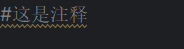
\includegraphics{3.1}
		\caption{行注释}
	\end{figure}
	
	
	块注释可以用多个\verb|#|、三单引号、三双引号
	
	\begin{figure}[H]
		\centering
		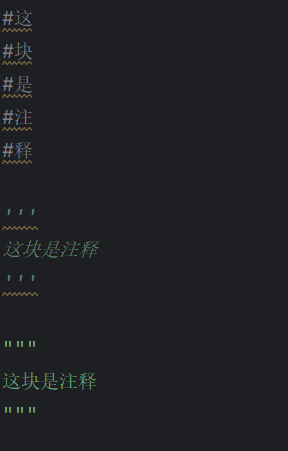
\includegraphics[scale=0.5]{3.2}
		\caption{块注释}
	\end{figure}
	
	2.输出语句
	在python中,用print输出语句,下面来输出一行helloworld
	\begin{figure}[H]
		\centering
		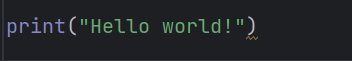
\includegraphics{3.3}
		\caption{helloworld}
	\end{figure}
	
	\begin{figure}[H]
		\centering
		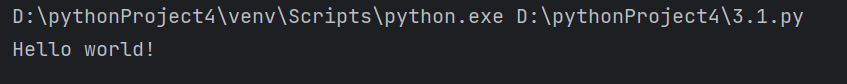
\includegraphics{3.4}
		\caption{helloworld}
	\end{figure}
	
	3.标识符
	
	(1)标识符的第一个字符必须是字母表中的字母或下划线
	
	(2)标识符的其他部分由字母、数字、下划线组成
	
	(3)标识符对大小写敏感
	
	
	\begin{figure}[H]
		\centering
		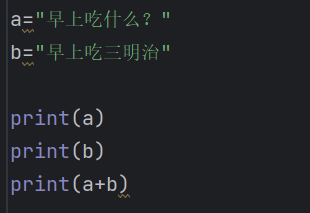
\includegraphics{3.5}
		\caption{标识符}
	\end{figure}
	
	
	\begin{figure}[H]
		\centering
		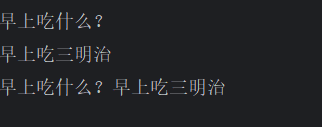
\includegraphics{3.6}
		\caption{标识符}
	\end{figure}
	
	4.多行语句
	
	在编写代码中,如果变量名很长,可以用反斜杠\verb|\|来实现多行语句。在\verb|[]、{}、()|里的多行语句,不需要使用反斜杠\verb|\|
	
	\begin{figure}[H]
		\centering
		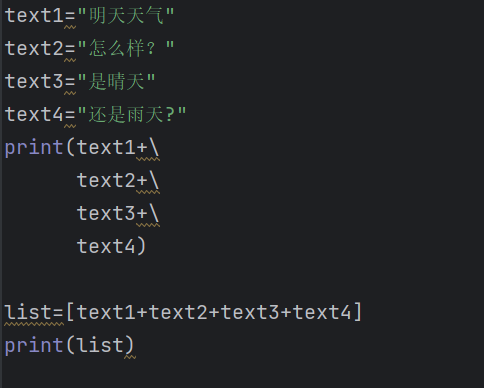
\includegraphics{3.7}
		\caption{多行语句}
	\end{figure}
	
	
	\begin{figure}[H]
		\centering
		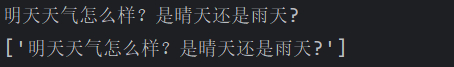
\includegraphics{3.8}
		\caption{多行语句}
	\end{figure}
	5.行与缩进
	
	在python中,用缩进来表示代码块,要保证正确的缩进
	
	6.关键字
	
	python中有33个关键字,其中False、None、True的首字母大写,其他还有\verb|class、finally、is、return、continue、for、lambda、try、def、from、nonlocal、while、and、del、global、not、with、as、elif、if、or、yield、assert、else、import、pass、break、except、in、raise|
	
	7.数据类型
	
	python中的数据类型有字符串、整型、列表、元组、字典、布尔型等。跟之前学过的c语言和c++不同,以整型为例:
	在python中有两种写法:
	
	counter = 100
	
	counter = int(100)
	
	浮点型、字符串型也类似
	
	布尔型是整型的子类型,只有两个取值——True和False,对应的整型分别为1和0
	
	8.运算符
	
	\begin{table}[h]
		\centering
		\caption{运算符}
		\begin{tabular}{|c|c|}
			\hline
			符号 & 描述  \\
			\hline
			== & 等于 \\
			\hline
			!= & 不等于\\
			\hline
			<= &小于等于\\ 
			\hline
			>= & 大于等于\\
			\hline
			>&大于\\
			\hline
			<&小于\\
			\hline
			and&与\\
			\hline
			or&或\\
			\hline
			not&非\\
			\hline
		\end{tabular}
	\end{table}
	
	关于逻辑运算:
	
	(1)与运算 and 一假则假
	
	(2)或运算 or 一真则真
	
	(3)非运算 not 真假倒转
	
	\subsubsection{导入包(库)}
	
	在python中用import或者from...import来导入相应的模块
	
	将整个模块(somemodule)导入,格式为: import somemodule
	
	从某个模块中导入某个函数,格式为: from somemodule import somefunction
	
	从某个模块中导入多个函数,格式为: from somemodule import firstfunc, secondfunc, thirdfunc
	
	将某个模块中的全部函数导入,格式为: from somemodule import *
	
	将某个模块改名(改为s),格式为:import somemodule as s
	\subsubsection{if语句}
	1.if判断语句 格式为:
	
	if:
	
	\quad \quad 执行语句
	
	下面是一个例子:
	
	\begin{figure}[H]
		\centering
		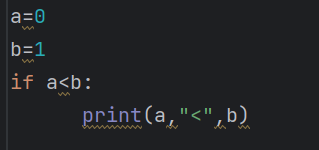
\includegraphics[scale=0.5]{3.9}
		\caption{if判断语句}
	\end{figure}
	
		\begin{figure}[H]
		\centering
		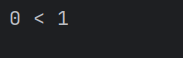
\includegraphics[scale=0.5]{3.10}
		\caption{if判断语句}
	\end{figure}
	
	2.if else分支语句 格式为:
	
	if:
	
	\quad \quad 执行语句
	
	else:
	
	\quad \quad 执行语句
	
	下面是一个例子:
	\begin{figure}[H]
		\centering
		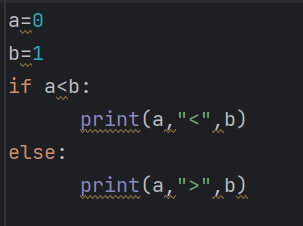
\includegraphics[scale=0.5]{3.11}
		\caption{if分支语句}
	\end{figure}
	
	\begin{figure}[H]
		\centering
		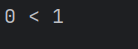
\includegraphics[scale=0.5]{3.12}
		\caption{if分支语句}
	\end{figure}
	
	3.if elif else多分支语句 格式为:
	
	if:
	
	\quad \quad 执行语句
	
	elif:
	
	\quad \quad 执行语句
	
	else:
	
	\quad \quad 执行语句
	
	下面是一个例子:
	
	\begin{figure}[H]
		\centering
		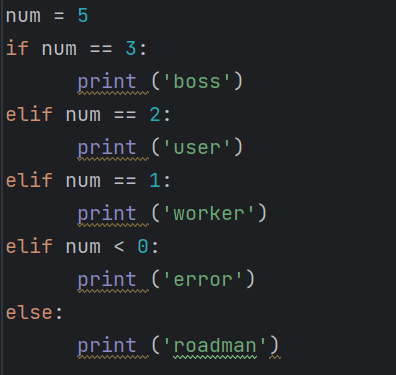
\includegraphics[scale=0.5]{3.13}
		\caption{if多分支语句}
	\end{figure}
	
	\begin{figure}[H]
		\centering
		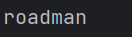
\includegraphics[scale=0.5]{3.14}
		\caption{if多分支语句}
	\end{figure}
	
	因为python不支持switch语句,所以多个条件判断,只能用 elif 来实现
	
	\subsubsection{循环语句 while、for、break、continue、pass}
	
	1.while循环语句
	
	(1)while循环语句
	
	下面是一个例子:
	
	\begin{figure}[H]
		\centering
		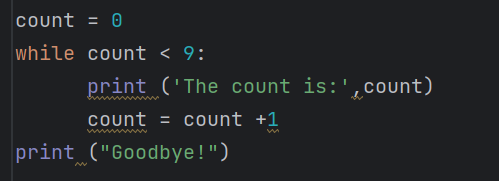
\includegraphics[scale=0.5]{3.15}
		\caption{while循环语句}
	\end{figure}
	
	\begin{figure}[H]
		\centering
		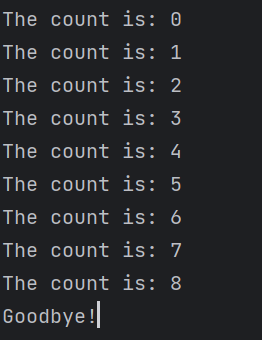
\includegraphics[scale=0.5]{3.16}
		\caption{while循环语句}
	\end{figure}
	
	
	(2)while循环语句else
	
	下面是一个例子:
	
	\begin{figure}[H]
		\centering
		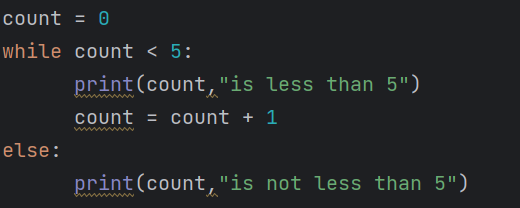
\includegraphics[scale=0.5]{3.17}
		\caption{while循环语句else}
	\end{figure}
	
	\begin{figure}[H]
		\centering
		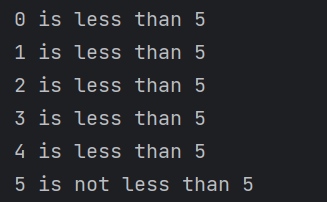
\includegraphics[scale=0.5]{3.18}
		\caption{while循环语句else}
	\end{figure}
	
	2.for循环
	
	(1)for循环语句
	
	下面是两个例子:
	
	\begin{figure}[H]
		\centering
		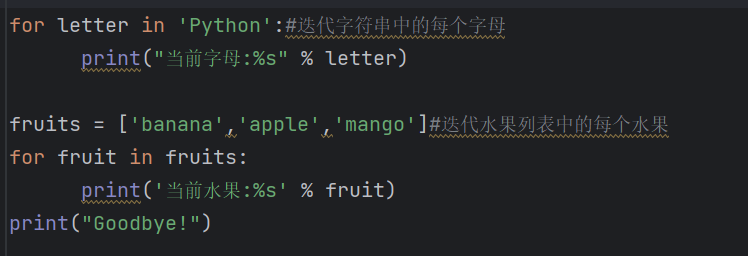
\includegraphics[scale=0.5]{3.19}
		\caption{for循环}
	\end{figure}
	
	\begin{figure}[H]
		\centering
		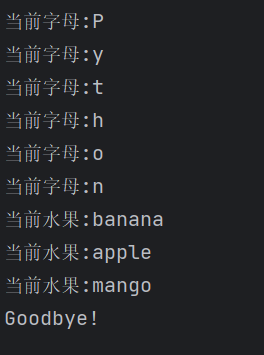
\includegraphics[scale=0.5]{3.20}
		\caption{for循环}
	\end{figure}
	
	(2)for循环语句else
	
	下面是一个例子:
	
	\begin{figure}[H]
		\centering
		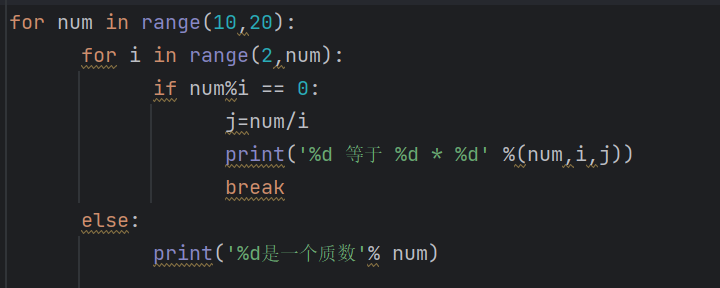
\includegraphics[scale=0.5]{3.21}
		\caption{for循环else}
	\end{figure}
	
	\begin{figure}[H]
		\centering
		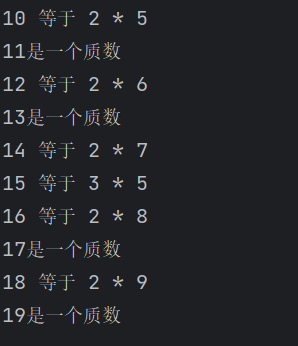
\includegraphics[scale=0.5]{3.22}
		\caption{for循环else}
	\end{figure}
	
	(3)break语句用来终止循环语句,而continue语句用来跳过当前循环的剩余语句,然后继续进行下一轮循环,此外还有一个pass语句,但是pass语句是空语句,不做任何事情,一般用做占位语句
	
	\subsubsection{数据类型和数据类型转换}
	
	整型int,长整型long,浮点型float,复数complex。其中,复数由实数部分和,虚数部分构成,可以用a+bj或者complex(a,b)表示,a是实部,b是虚部。
	
	数据类型转换:
	
	int(x) 将x转换为一个整数
	
	long(x) 将x转换为一个长整数
	
	float(x) 将x转换为一个浮点数
	
	str(x) 将x转换为字符串
	
	list(s) 将序列s转换为一个列表
	
	
	...
	
	\subsubsection{字符串}
	
	字符串是python中最常用的数据类型,使用单引号或双引号来创建字符串。python不支持单字符类型,单字符在python中也是作为一个字符串使用。python访问子字符串,可以用方括号[]来截取字符串。
	
	\begin{table}[h]
		\centering
		\caption{字符串运算符}
		\begin{tabular}{|c|p{10cm}|}
			\hline
			符号 & 描述  \\
			\hline
			+ & 字符串连接 \\
			\hline
			* & 重复输出字符串\\
			\hline
			[] &通过索引获取字符串中字符\\ 
			\hline
			[:] & 截取字符串中的一部分,遵循左闭右开原则,例如str[0:2]是不包含第3个字符的\\
			\hline
			in&成员运算符—如果字符串中包含给定的字符返回True\\
			\hline
			not in&成员运算符—如果字符串中不包含给定的字符串返回True\\
			\hline
			r/R&原始字符串 - 原始字符串:所有的字符串都是直接按照字面的意思来使用,没有转义特殊或不能打印的字符。 原始字符串除在字符串的第一个引号前加上字母 r(可以大小写)以外,与普通字符串有着几乎完全相同的语法。\\
			\hline
		\end{tabular}
	\end{table}
	
	下面是一些例子:
	
	\begin{figure}[H]
		\centering
		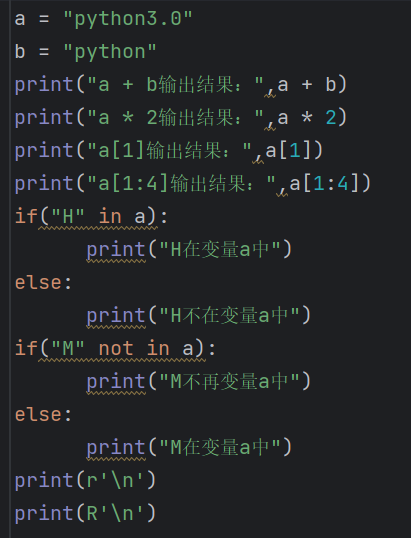
\includegraphics[scale=0.5]{3.23}
		\caption{字符串运算符}
	\end{figure}
	
	\begin{figure}[H]
		\centering
		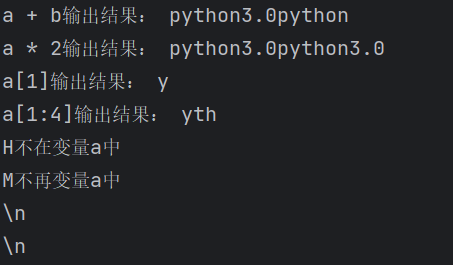
\includegraphics[scale=0.5]{3.24}
		\caption{字符串运算符}
	\end{figure}
	
	\subsubsection{列表}
	列表的数据项不需要具有相同的类型,下面是一个列表:
	
	\begin{figure}[H]
		\centering
		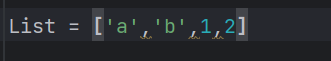
\includegraphics{3.25}
		\caption{列表}
	\end{figure}
	
	索引:序列中的每个值都有对应的位置值,称之为索引,第一个索引是 0,第二个索引是 1,索引也可以从尾部(负索引)开始,最后一个元素的索引为 -1,往前一位为 -2,以此类推。
	
	\begin{figure}[H]
		\centering
		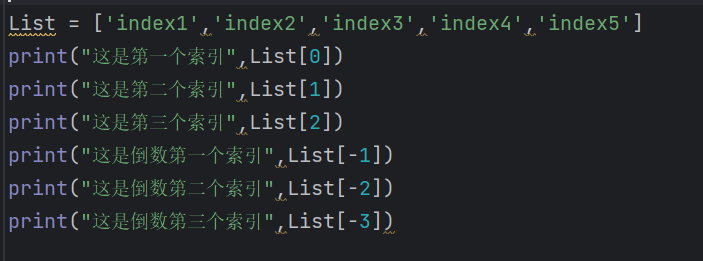
\includegraphics[scale=0.5]{3.26}
		\caption{索引}
	\end{figure}
	
	\begin{figure}[H]
		\centering
		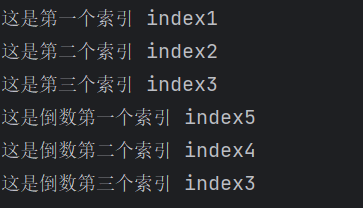
\includegraphics[scale=0.5]{3.27}
		\caption{索引}
	\end{figure}
	
	切片:使用方括号[]截取字符
	
	\begin{figure}[H]
		\centering
		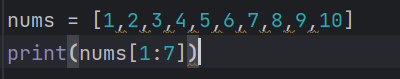
\includegraphics[scale=0.5]{3.28}
		\caption{切片}
	\end{figure}
	
	\begin{figure}[H]
		\centering
		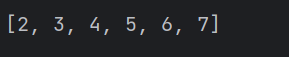
\includegraphics[scale=0.5]{3.29}
		\caption{切片}
	\end{figure}
	
	添加:使用append()方法来添加列表项
	
	\begin{figure}[H]
		\centering
		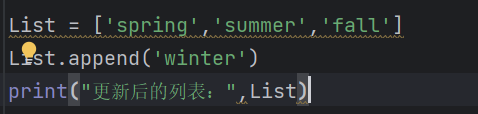
\includegraphics[scale=0.5]{3.30}
		\caption{添加}
	\end{figure}
	
	\begin{figure}[H]
		\centering
		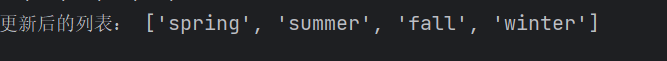
\includegraphics[scale=0.5]{3.31}
		\caption{添加}
	\end{figure}
	
	删除:使用del语句来删除列表元素
	
	\begin{figure}[H]
		\centering
		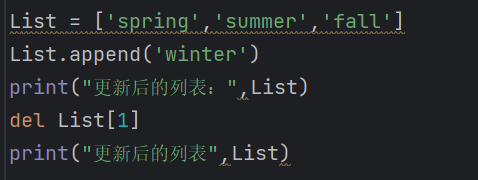
\includegraphics[scale=0.5]{3.32}
		\caption{删除}
	\end{figure}
	
	\begin{figure}[H]
		\centering
		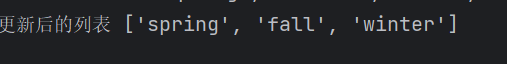
\includegraphics[scale=0.5]{3.33}
		\caption{删除}
	\end{figure}
	
	\subsubsection{元组}
	元组与列表类似,不同之处在于元组的元素不能修改。元组使用小括号(),列表使用方括号[]
	
	索引:元组使用下标索引来访问元组中的值
	
	\begin{figure}[H]
		\centering
		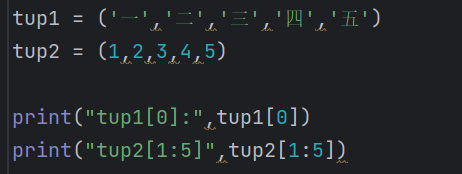
\includegraphics[scale=0.5]{3.34}
		\caption{索引}
	\end{figure}
	
	\begin{figure}[H]
		\centering
		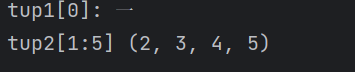
\includegraphics[scale=0.5]{3.35}
		\caption{索引}
	\end{figure}
	
	修改:
	
	\begin{figure}[H]
		\centering
		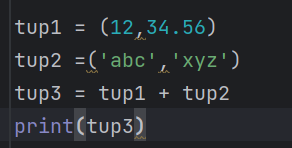
\includegraphics[scale=0.5]{3.36}
		\caption{修改}
	\end{figure}
	
	\begin{figure}[H]
		\centering
		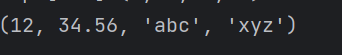
\includegraphics[scale=0.5]{3.37}
		\caption{修改}
	\end{figure}
	
	删除:元组中的元素是不允许删除的,但我们可以使用del语句来删除整个元组
	
	\begin{figure}[H]
		\centering
		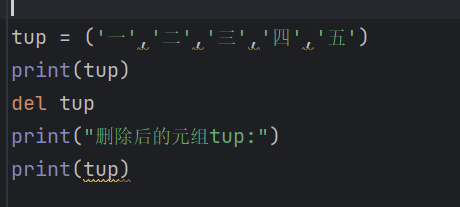
\includegraphics[scale=0.5]{3.38}
		\caption{删除}
	\end{figure}
	
	\begin{figure}[H]
		\centering
		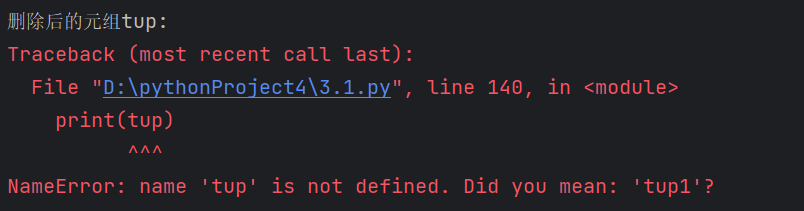
\includegraphics[scale=0.5]{3.39}
		\caption{删除}
	\end{figure}
	
	通过报错信息可以看到,元组已经被删除,已经没有这个元组了。
	
	元组同样也可以使用+和*来进行运算,还可以索引,截取。
	
	同时,元组还有内置函数:
	
	\begin{table}[h]
		\centering
		\caption{元组内置函数}
		\begin{tabular}{|c|p{10cm}|}
			\hline
			符号 & 描述  \\
			\hline
			len(tuple) & 计算元组元素个数 \\
			\hline
			max(tuple) & 返回元组中元素最大值\\
			\hline
			min(tuple) &返回元组中元素最小值\\ 
			\hline
			tuple(iterable) & 将可迭代系列转换为元组\\
			\hline
		\end{tabular}
	\end{table}
	
	下面是一些例子:
	
	\begin{figure}[H]
		\centering
		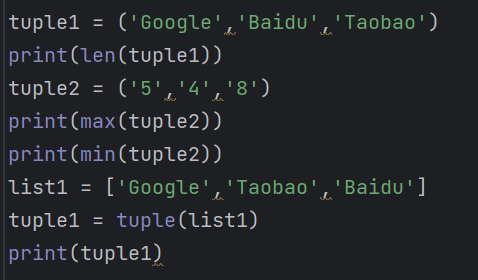
\includegraphics[scale=0.5]{3.40}
		\caption{元组内置函数}
	\end{figure}
	
	\begin{figure}[H]
		\centering
		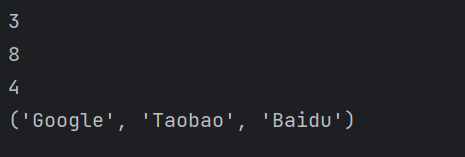
\includegraphics[scale=0.5]{3.41}
		\caption{元组内置函数}
	\end{figure}
	
	\subsubsection{字典}
	字典是另一种可变容器模型,可存储任意类型对象。字典中的每个键值key=>value对用冒号:分割,每个对之间用逗号,分割,整个字典包括在花括号{}中。
	
	下面是一个字典:
	\begin{figure}[H]
		\centering
		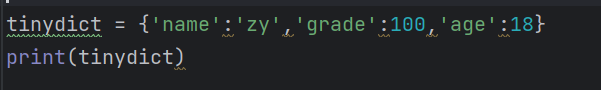
\includegraphics[scale=0.5]{3.42}
		\caption{字典}
	\end{figure}
	
	\begin{figure}[H]
		\centering
		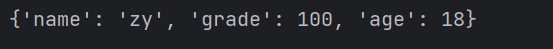
\includegraphics[scale=0.5]{3.43}
		\caption{字典}
	\end{figure}
	
	如果要访问字典里的值,把相应键放入到方括号中:
	
	\begin{figure}[H]
		\centering
		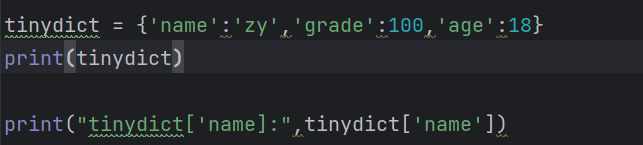
\includegraphics[scale=0.5]{3.44}
		\caption{访问字典}
	\end{figure}
	
	\begin{figure}[H]
		\centering
		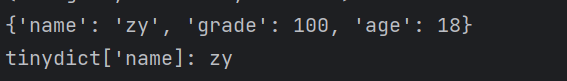
\includegraphics[scale=0.5]{3.45}
		\caption{访问字典}
	\end{figure}
	
	
	修改字典:向字典添加新内容的方法是增加新的键/值对,修改或删除已有键/值对
	
	\begin{figure}[H]
		\centering
		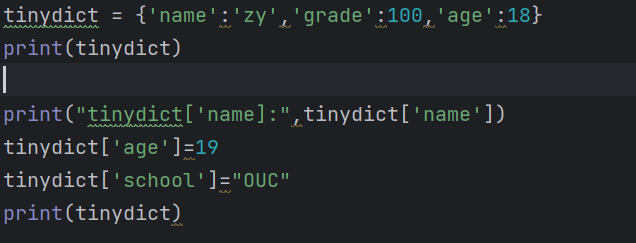
\includegraphics[scale=0.5]{3.46}
		\caption{修改字典}
	\end{figure}
	
	\begin{figure}[H]
		\centering
		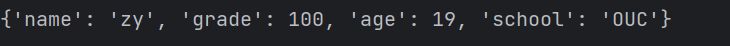
\includegraphics[scale=0.5]{3.47}
		\caption{修改字典}
	\end{figure}
	
	清空字典用.clear(),删除一个键用del
	
	\begin{figure}[H]
		\centering
		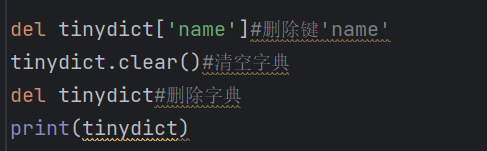
\includegraphics[scale=0.5]{3.48}
		\caption{字典}
	\end{figure}
	
	下面是字典内置函数:
	
	\begin{table}[h]
		\centering
		\caption{字典内置函数}
		\begin{tabular}{|c|p{10cm}|}
			\hline
			符号 & 描述  \\
			\hline
			len(dict) & 计算字典元素个数,即键的总数 \\
			\hline
			str(dict) & 输出字典,可以打印的字符串表示\\
			\hline
			type(variable) &返回输入的变量类型,如果变量是字典就返回字典类型\\ 
			\hline
		\end{tabular}
	\end{table}
	
	下面是例子:
	\begin{figure}[H]
		\centering
		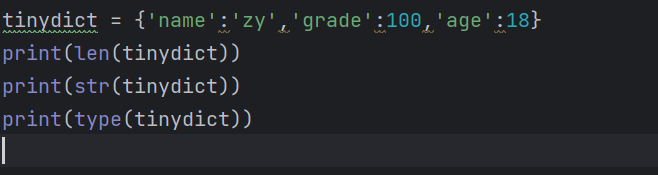
\includegraphics[scale=0.5]{3.49}
		\caption{字典函数}
	\end{figure}
	
		\begin{figure}[H]
		\centering
		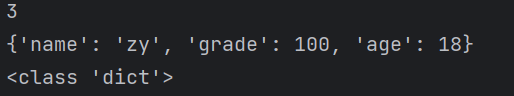
\includegraphics[scale=0.5]{3.50}
		\caption{字典函数}
	\end{figure}
	
	\subsubsection{集合}
	集合(set)是一个无序的不重复元素序列。
	集合其实也可以看作是一个没有键,只有值的字典。
	
	假设现在有两个集合a、b
	
	\verb|a-b|(集合a中包含而集合b中不包含的元素)
	
	a|b(集合a或b中包含的所有元素)
	
	\verb|a&b|(集合a和b中都包含了的元素)
	
	\verb|a^b|(不同时包含于a和b的元素)
	
	同时输出结果不是固定的,是个无序的不重复元素序列。
	
	\begin{figure}[H]
		\centering
		\includegraphics[scale=0.5]{3.51}
		\caption{集合}
	\end{figure}
	
	\begin{figure}[H]
		\centering
		\includegraphics[scale=0.5]{3.52}
		\caption{集合}
	\end{figure}
	
	集合中常用的几个方法:
	
	\begin{table}[h]
		\centering
		\caption{集合}
		\begin{tabular}{|c|p{10cm}|}
			\hline
			符号 & 描述  \\
			\hline
			add() & 将元素添加到集合中,如果元素已存在,则不进行任何操作 \\
			\hline
			update() & 添加元素,且参数可以是列表,元组,字典等\\
			\hline
			remove() &将元素从集合中移除,如果元素不存在,则会发生错误\\ 
			\hline
			discard() & 将元素从集合中移除,且如果元素不存在,不会发生错误\\
			\hline
			pop()&将集合进行无序的排列,然后将这个无序排列集合的左面第一个元素进行删除\\
			\hline
			len()&计算集合元素个数\\
			\hline
			clear()&清空集合\\
			\hline
			in & 判断元素是否在集合中,存在返回True,不存在返回False\\
			\hline
		\end{tabular}
	\end{table}
	
	下面是一些例子:
	
	\begin{figure}[H]
		\centering
		\includegraphics[scale=0.5]{3.53}
		\caption{集合}
	\end{figure}
	
	\begin{figure}[H]
		\centering
		\includegraphics[scale=0.5]{3.54}
		\caption{集合}
	\end{figure}
	
	\subsubsection{迭代器与生成器}
	
	迭代器是一个可以记住遍历的位置的对象。迭代器对象从集合的第一个元素开始访问,直到所有的元素被访问结束。迭代器只能往前不会后退。
	迭代器有两个基本的方法:iter() 和 next() 。
	字符串,列表或元组对象都可用于创建迭代器。
	迭代器对象可以使用常规for语句、while语句等进行遍历。
	
	下面是一个例子:
	
	\begin{figure}[H]
	    \centering
	    \includegraphics[scale=0.5]{3.55}
	    \caption{迭代器}
    \end{figure}

    \begin{figure}[H]
	    \centering
	    \includegraphics[scale=0.5]{3.56}
	    \caption{迭代器}
    \end{figure}
    
    Stoplteration异常用于标识迭代的完成,防止出现无限循环的情况。在 next() 方法中我们可以设置在完成指定循环次数后触发 StopIteration 异常来结束迭代。下面是一个迭代二十次停止执行的例子:
    
    \begin{figure}[H]
    	\centering
    	\includegraphics[scale=0.5]{3.57}
    	\caption{Stoplteration}
    \end{figure}
    
    \begin{figure}[H]
    	\centering
    	\includegraphics[scale=0.5]{3.58}
    	\caption{Stoplteration}
    \end{figure}

	生成器:使用yield的函数被成为生成器。其实生成器也是一个迭代器。在调用生成器运行的过程中,每次遇到 yield 时函数会暂停并保存当前所有的运行信息,返回 yield 的值, 并在下一次执行 next() 方法时从当前位置继续运行。调用一个生成器函数,返回的是一个迭代器对象。
	
	下面是一个例子实现斐波那契数列:
	
	\begin{figure}[H]
		\centering
		\includegraphics[scale=0.5]{3.59}
		\caption{斐波那契数列}
	\end{figure}
	
	\begin{figure}[H]
		\centering
		\includegraphics[scale=0.5]{3.60}
		\caption{斐波那契数列}
	\end{figure}
	
	\subsubsection{日期}
	python提供了一个time和calendar模块可以用于格式化日期和时间。time模块下有很多函数可以转换常见日期格式,函数time.time()用于获取当前时间戳。
	
	\begin{figure}[H]
		\centering
		\includegraphics[scale=0.5]{3.61}
		\caption{时间戳}
	\end{figure}
	
	\begin{figure}[H]
		\centering
		\includegraphics[scale=0.5]{3.62}
		\caption{时间戳}
	\end{figure}
	
	可以使用time模块的strftime方法来格式化日期:
	
	\begin{figure}[H]
		\centering
		\includegraphics[scale=0.5]{3.63}
		\caption{格式化日期}
	\end{figure}
	
	\begin{figure}[H]
		\centering
		\includegraphics[scale=0.5]{3.64}
		\caption{格式化日期}
	\end{figure}
	
	\subsubsection{函数}
	函数以def关键词开头,后面是函数名和括号,括号里面是要传入的参数。使用return结束函数。在下面直接用函数名调用函数。
	
	\begin{figure}[H]
		\centering
		\includegraphics[scale=0.5]{3.65}
		\caption{函数}
	\end{figure}
	
	\begin{figure}[H]
		\centering
		\includegraphics[scale=0.5]{3.66}
		\caption{函数}
	\end{figure}
	
	\subsubsection{文件}
	
	打开文件用open()函数,关闭用close()函数。write()方法可以将任何字符串写入一个打开的文件,read()方法可以从一个打开的文件中读取一个字符串。下面是一个例子:
	
	\begin{figure}[H]
		\centering
		\includegraphics[scale=0.5]{3.67}
		\caption{文件}
	\end{figure}
	
	\begin{figure}[H]
		\centering
		\includegraphics[scale=0.5]{3.68}
		\caption{文件}
	\end{figure}
	
	
	
	
	\subsubsection{os模块}
	
	python的os模块提供了执行文件操作的方法,比如重命名和删除文件。要使用这个模块,要先导入它,然后才可以调用相关功能。使用\verb|import os|语句导入。
	
	重命名是rename()方法,它需要两个参数,当前的文件名和新文件名。删除文件用remove()方法,需要提供要删除的文件名作为参数。
	下面是一个将我之前创建的foo文件重命名为foo1的操作:
	\begin{figure}[H]
		\centering
		\includegraphics[scale=0.5]{3.69}
		\caption{重命名}
	\end{figure}
	
	\begin{figure}[H]
		\centering
		\includegraphics[scale=0.5]{3.70}
		\caption{重命名}
	\end{figure}
	
	可以看到,重命名成功。
	
	下面我来删除这个文件:
	\begin{figure}[H]
		\centering
		\includegraphics[scale=0.5]{3.71}
		\caption{删除}
	\end{figure}
	然后到原来文件所在的目录就可以看到这个文件已经没有了。
	
	\subsubsection{面向对象}
	下面简单介绍类:
	
	使用class语句创建一个新类,类之后为类的名称并以冒号结尾。下面用一个实例来具体介绍:
	
	\begin{figure}[H]
		\centering
		\includegraphics[scale=0.5]{3.72}
		\caption{类}
	\end{figure}
	
	\begin{figure}[H]
		\centering
		\includegraphics[scale=0.5]{3.73}
		\caption{类}
	\end{figure}
	
	\verb|__init__|方法是一种特殊的方法,被称为类的构造函数或初始化方法,当创建了这个类的实例时就会调用该方法
	self 代表类的实例,self 在定义类的方法时是必须有的,虽然在调用时不必传入相应的参数。其他的创建和访问属性都和c和c++相似。
	
	
	
	\subsection{python计算机视觉}
	\subsubsection{PIL:Python图像处理类库}
	下面使用convert()方法将一个图片转换成灰色
	\begin{figure}[H]
		\centering
		\includegraphics[scale=0.5]{3.83}
		\caption{灰色}
	\end{figure}
	
	\begin{figure}[H]
		\centering
		\includegraphics[scale=0.05]{3.81}
		\caption{原图片}
	\end{figure}
	
	\begin{figure}[H]
		\centering
		\includegraphics[scale=0.05]{3.80}
		\caption{灰色图片}
	\end{figure}
	\subsubsection{Matplotlib}
	下面在原图上绘制几个点和一条线段:
	\begin{figure}[H]
		\centering
		\includegraphics[scale=0.10]{3.91}
		\caption{原图片}
	\end{figure}
	
	\begin{figure}[H]
		\centering
		\includegraphics[scale=0.50]{3.92}
		\caption{方法}
	\end{figure}
	
	绘制后的图片:
	\begin{figure}[H]
		\centering
		\includegraphics[scale=0.50]{3.90}
		\caption{图片1}
	\end{figure}
	如果不想显示坐标轴,增加axis('off'),下面是改进后的图片:
	\begin{figure}[H]
		\centering
		\includegraphics[scale=0.50]{3.94}
		\caption{图片2}
	\end{figure}
	\subsubsection{NumPy将图像转化为数组}
	将图片转化为数组:
	\begin{figure}[H]
		\centering
		\includegraphics[scale=0.50]{3.95}
		\caption{数组}
	\end{figure}
	
	\begin{figure}[H]
		\centering
		\includegraphics[scale=0.50]{3.96}
		\caption{数组}
	\end{figure}
	
	其中因为图像通常被编码成无符号八位整型,所以在第一种情况下,数组的数据类型为"unit8"。在第二种情况下,对图像进行灰度化处理,并且在创建数组时使用额外的参数“f”;该
	参数将数据类型转换为浮点型float32。
	\subsubsection{SciPy图像模糊}
	下面进行模糊图片:
	
	\begin{figure}[H]
		\centering
		\includegraphics[scale=0.50]{3.98}
		\caption{模糊图片}
	\end{figure}
	\begin{figure}[H]
		\centering
		\includegraphics[scale=0.10]{3.99}
		\caption{模糊图片}
	\end{figure}
	
	
	\section{心得体会}
	本次学习主要学习了python,并了解了一些python计算机视觉的相干内容,通过使用 PIL 处理图像、numpy 进行数值操作以及 scipy.ndimage 的高斯滤波等,我掌握了图像的基本处理技术,很有收获。
	\section{相关练习、报告和代码查看链接}
	本次报告相关练习、报告和代码均可以在https://kkgithub.com/zhangtantan77/work查看

\end{document}